%
% $Id: slides.tex 4228 2006-06-21 21:55:12Z jjamor $
%
%
% Compilar a .pdf con LaTeX (pdflatex)
% Es necesario instalar Beamer (paquete latex-beamer en Debian)
%

%
% Gráficos:
% Los gráficos pueden suministrarse en PNG, JPG, TIF, PDF, MPS
% Los EPS deben convertirse a PDF (usar epstopdf)
%

\documentclass{beamer}
\usetheme{Warsaw}
\usebackgroundtemplate{
\includegraphics[width=\paperwidth]{format/opensistemas-bg.png}}
\usepackage[spanish]{babel}
\usepackage[utf8]{inputenc}
\usepackage{graphics}
\usepackage{amssymb} % Simbolos matematicos
\usepackage{url}

%\definecolor{libresoftgreen}{RGB}{162,190,43}
%\definecolor{libresoftblue}{RGB}{0,98,143}

%\setbeamercolor{titlelike}{bg=libresoftgreen}

%% Metadatos del PDF.
\hypersetup{
  pdftitle={FLOSS Leaders},
  pdfauthor={J.J. Amor, M. Vidal, F. Ortega, P. Coca},
  pdfcreator={GSyC/Libresoft},
  pdfproducer=PDFLaTeX,
  pdfsubject={nn},
}
%%


\AtBeginSection[]
{
  \begin{frame}<presentation>
    \frametitle{Index}
    \tableofcontents[current]
  \end{frame}
}


\begin{document}

\title{FLOSS Leaders}
\subtitle{Master on Free Software}
% \institute{\\jjamor@opensistemas.com\\
% Open Sistemas}
\author{J.J. Amor, M. Vidal, F. Ortega, P. Coca}
\date{4 de noviembre de 2011}

\frame{
\maketitle
\begin{center}

\includegraphics[width=6cm]{format/gsyc-open-urjc}
\end{center}
}


% Si el titulo o el autor se quieren acortar para los pies de p�gina
% se pueden redefinir aqu�:
%\title{Titulo corto}
%\author{Autores abreviado}


%% LICENCIA DE REDISTRIBUCION DE LAS TRANSPAS
\frame{
~
\vspace{4cm}

\begin{flushright}
{\tiny
(cc) 2010-2011 Juanjo Amor, Miguel Vidal, Felipe Ortega, Pedro Coca. \\
Some rights reserved. This document is distributed under the Creative \\
            Commons Attribution-ShareAlike 3.0 licence, available in \\
            http://creativecommons.org/licenses/by-sa/3.0/

%  Este documento (o uno muy similar) está disponible en \\
%  \url{http://gsyc.escet.urjc.es/~jjamor/}
}
\end{flushright}
}
%%

%%%%%%
%Transpas separadas por \begin{frame}
%%%%%%%%%%%%%%%%%%%%%%%%\end{frame}

\section{Introduction}

\begin{frame}
\frametitle{Introduction}
\begin{itemize}
\item FLOSS history and Computer science history are very parallel.
\pause
\item Because, in the beginning, first computers always were ``open sourced''.
\pause
\item For example, in the 60s, software was acompanying hardware, and source code could be modified by anyone...
\pause
\item ... and shared with others.
\end{itemize}
\end{frame}

%%%%%%%%%%%%%%%%%%%%%%%%%%%%%%%%%%%%%%%%%%%%%%%%%%%%%%%%%%%%%%
\begin{frame}
\frametitle{Introduction}
\begin{itemize}
\item In these days, some scientists appeared, related with first commercial computers.
\pause
\item Engineers and physicists appeared with high interests in ``how it works''.
\pause
\item These people were truly entusiasts, people which created and modified software for enjoying them.
\pause
\item These were called ``real programmers''.
\item ``A brief history of hackerdom'', Eric S. Raymond.
\url{http://www.catb.org/~esr/writings/cathedral-bazaar/hacker-history/} 
\end{itemize}
\end{frame}
%%%%%%%%%%%%%%%%%%%%%%%%%%%%%%%%%%%%%%%%%%%%%%%%%%%%%%%%%%%%%%

%%%%%%%%%%%%%%%%%%%%%%%%%%%%%%%%%%%%%%%%%%%%%%%%%%%%%%%%%%%%%%
\begin{frame}
\frametitle{Introduction}
\begin{itemize}
\item Since these days to today, FLOSS culture (and technology) evolution has been always driven by some people.
\pause
\item People with name and surname which have contributed something crucial for that moment.
\pause
\item These people will be called by us ``{\bf FLOSS Leaders}''.
\end{itemize}
\end{frame}
%%%%%%%%%%%%%%%%%%%%%%%%%%%%%%%%%%%%%%%%%%%%%%%%%%%%%%%%%%%%%%

%%%%%%%%%%%%%%%%%%%%%%%%%%%%%%%%%%%%%%%%%%%%%%%%%%%%%%%%%%%%%%
\begin{frame}
\frametitle{Overview of this unit}
\begin{itemize}
\item In this unit, we will see, in historical order, some key people in libre software field.
\item This unit will be organised in an interactive manner:
\item First, we will give you some names and photographs...
\item ... and you will be the responsible of investigate all about them.
\item The exercises will consist in, preparation of a slides presentation with the information you have investigated.
\end{itemize}
\end{frame}
%%%%%%%%%%%%%%%%%%%%%%%%%%%%%%%%%%%%%%%%%%%%%%%%%%%%%%%%%%%%%%

\section{FLOSS Leaders}

%%%%%%%%%%%%%%%%%%%%%%%%%%%%%%%%%%%%%%%%%%%%%%%%%%%%%%%%%%%%%%
\begin{frame}
\frametitle{FLOSS Leader}

\begin{figure}[h]
\begin{center}
  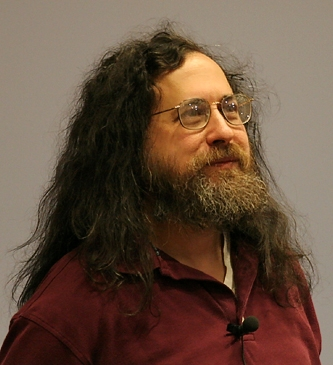
\includegraphics[height=1.80in]{figs/rms.jpg}
%  \caption{{\footnotesize Linus Torvalds}}
\end{center}
\end{figure}

\pause

\begin{center}
{\it Richard M. Stallman}
\end{center}

\end{frame}
%%%%%%%%%%%%%%%%%%%%%%%%%%%%%%%%%%%%%%%%%%%%%%%%%%%%%%%%%%%%%%

%%%%%%%%%%%%%%%%%%%%%%%%%%%%%%%%%%%%%%%%%%%%%%%%%%%%%%%%%%%%%%
\begin{frame}
\frametitle{FLOSS Leader}

Some ideas to find information about this leader.
\pause
\begin{itemize}
\item A short bio.
\item His most known project and how it was conceived.
\item How is he making a living today?
\item Evolution of participation on the project.
\item How can we contact him? Did he use social networks?
\item \ldots
\end{itemize}

\end{frame}

%%%%%%%%%%%%%%%%%%%%%%%%%%%%%%%%%%%%%%%%%%%%%%%%%%%%%%%%%%%%%%
\begin{frame}
\frametitle{FLOSS Leader}

\begin{figure}[h]
\begin{center}
  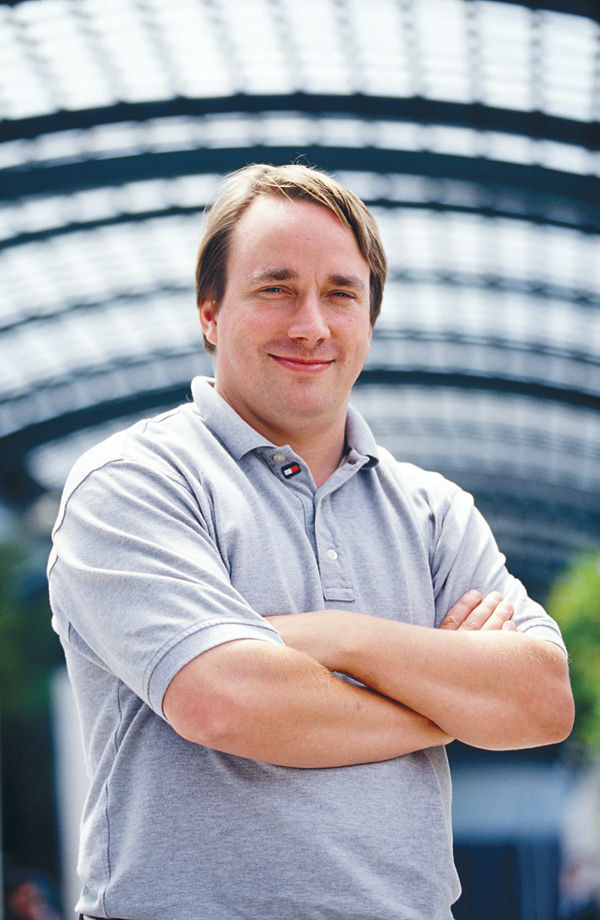
\includegraphics[height=1.80in]{figs/linus_torvalds.jpg}
%  \caption{{\footnotesize Linus Torvalds}}
\end{center}
\end{figure}

\pause

\begin{center}
{\it Linus Torvalds}
\end{center}

\end{frame}

%%%%%%%%%%%%%%%%%%%%%%%%%%%%%%%%%%%%%%%%%%%%%%%%%%%%%%%%%%%%%%
\begin{frame}
\frametitle{FLOSS Leader}

Some ideas to find information about this leader.
\pause
\begin{itemize}
\item A short bio.
\item The history of Linux.
\item Professional activities after creating Linux.
\item How is he making a living today?
\item \ldots
\end{itemize}

\end{frame}

%%%%%%%%%%%%%%%%%%%%%%%%%%%%%%%%%%%%%%%%%%%%%%%%%%%%%%%%%%%%%%
\begin{frame}
\frametitle{FLOSS Leader}

\begin{figure}[h]
\begin{center}
  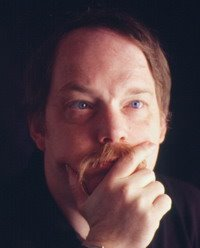
\includegraphics[height=1.80in]{figs/esr.jpg}
%  \caption{{\footnotesize Linus Torvalds}}
\end{center}
\end{figure}

\pause

\begin{center}
{\it Eric S. Raymond}
\end{center}

\end{frame}


%%%%%%%%%%%%%%%%%%%%%%%%%%%%%%%%%%%%%%%%%%%%%%%%%%%%%%%%%%%%%%
\begin{frame}
\frametitle{FLOSS Leader}

Some ideas to find information about this leader.
\pause
\begin{itemize}
\item A short bio.
\item Well known software he developed.
\item Projects he co-founded.
\item His most known essay.
\item Anecdotes\ldots
\end{itemize}

\end{frame}

%%%%%%%%%%%%%%%%%%%%%%%%%%%%%%%%%%%%%%%%%%%%%%%%%%%%%%%%%%%%%%
\begin{frame}
\frametitle{FLOSS Leader}

\begin{figure}[h]
\begin{center}
  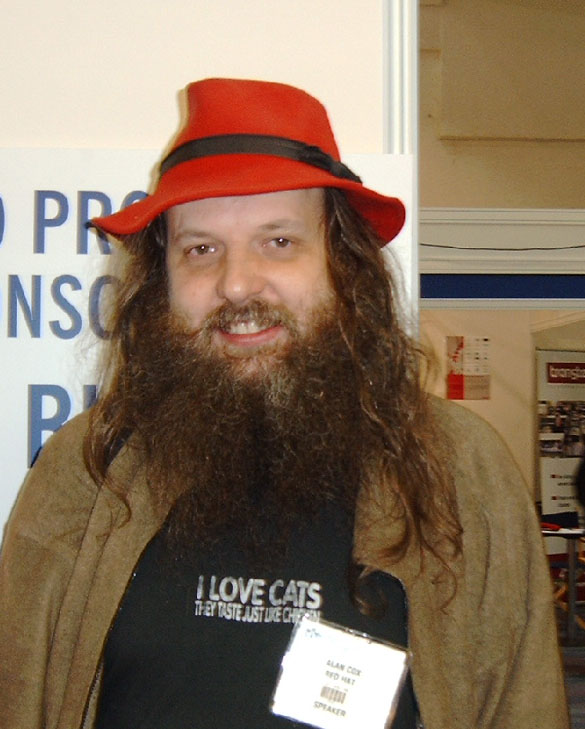
\includegraphics[height=1.80in]{figs/AlanCox.png}
%  \caption{{\footnotesize Linus Torvalds}}
\end{center}
\end{figure}

\pause

\begin{center}
{\it Alan Cox}
\end{center}

\end{frame}

%%%%%%%%%%%%%%%%%%%%%%%%%%%%%%%%%%%%%%%%%%%%%%%%%%%%%%%%%%%%%%
\begin{frame}
\frametitle{FLOSS Leader}

Some ideas to find information about this leader.
\pause
\begin{itemize}
\item A short bio.
\item Alan Cox and Linux.
\item Other projects.
\item How is he making a living today?
\item \ldots
\end{itemize}

\end{frame}

%%%%%%%%%%%%%%%%%%%%%%%%%%%%%%%%%%%%%%%%%%%%%%%%%%%%%%%%%%%%%%
\begin{frame}
\frametitle{FLOSS Leader}

\begin{figure}[h]
\begin{center}
  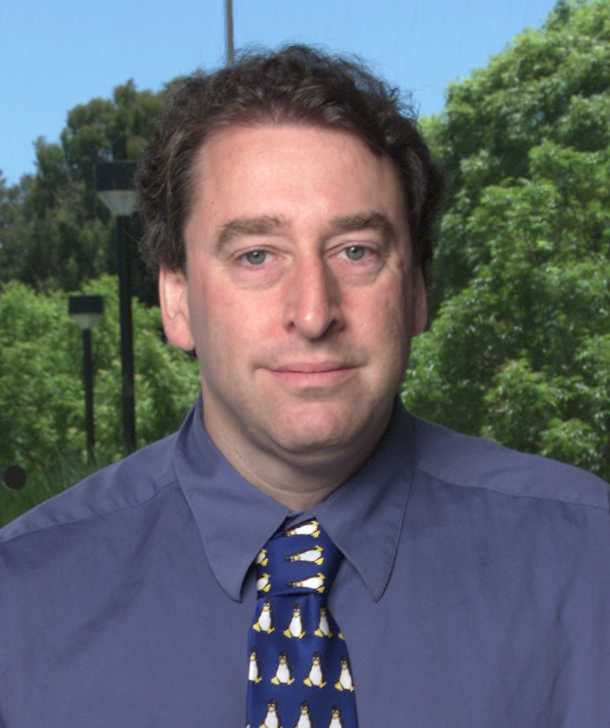
\includegraphics[height=1.80in]{figs/bruceperens.jpg}
%  \caption{{\footnotesize Linus Torvalds}}
\end{center}
\end{figure}

\pause

\begin{center}
{\it Bruce Perens}
\end{center}

\end{frame}

%%%%%%%%%%%%%%%%%%%%%%%%%%%%%%%%%%%%%%%%%%%%%%%%%%%%%%%%%%%%%%
\begin{frame}
\frametitle{FLOSS Leader}

Some ideas to find information about this leader.
\pause
\begin{itemize}
\item A short bio.
\item Which organization he proposed?
\item All about Debian Social Contract...
\item Linux and the enterprise world.
\item How is he making a living today?
\item \ldots
\end{itemize}

\end{frame}

%%%%%%%%%%%%%%%%%%%%%%%%%%%%%%%%%%%%%%%%%%%%%%%%%%%%%%%%%%%%%%
%%%%%%%%%%%%%%%%%%%%%%%%%%%%%%%%%%%%%%%%%%%%%%%%%%%%%%%%%%%%%%
\begin{frame}
\frametitle{FLOSS Leader}

\begin{figure}[h]
\begin{center}
  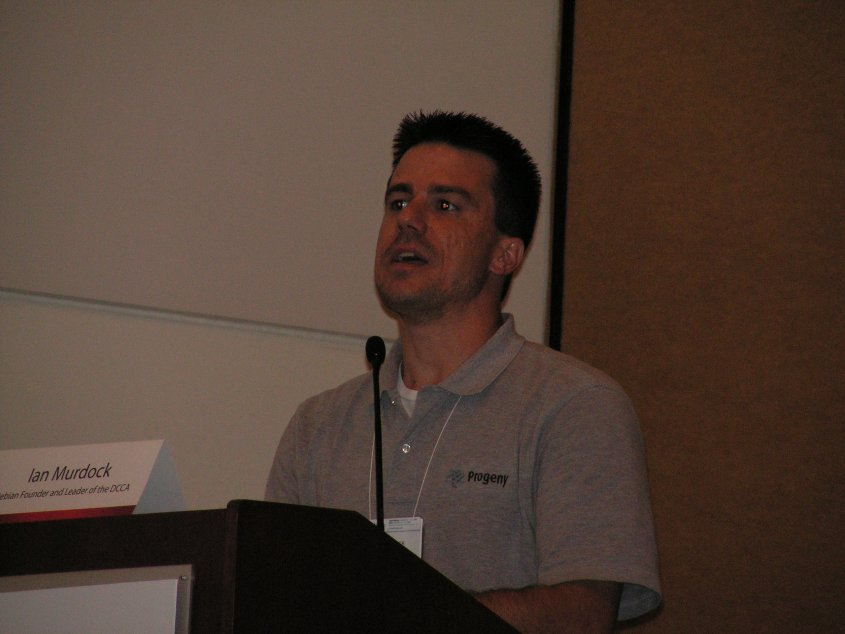
\includegraphics[height=1.80in]{figs/ian_murdock.jpg}
%  \caption{{\footnotesize Linus Torvalds}}
\end{center}
\end{figure}

\pause

\begin{center}
{\it Ian Murdock}
\end{center}

\end{frame}

%%%%%%%%%%%%%%%%%%%%%%%%%%%%%%%%%%%%%%%%%%%%%%%%%%%%%%%%%%%%%%
\begin{frame}
\frametitle{FLOSS Leader}

Some ideas to find information about this leader.
\pause
\begin{itemize}
\item A short bio.
\item What is ``Debian''? And what was the origin of the name?
\item The project co-founded with Bruce Perens.
\item Later enterprises related to Debian.
\item Only Debian?
\item How is he making a living today?
\item \ldots
\end{itemize}

\end{frame}

%%%%%%%%%%%%%%%%%%%%%%%%%%%%%%%%%%%%%%%%%%%%%%%%%%%%%%%%%%%%%%
%%%%%%%%%%%%%%%%%%%%%%%%%%%%%%%%%%%%%%%%%%%%%%%%%%%%%%%%%%%%%%
\begin{frame}
\frametitle{FLOSS Leader}

\begin{figure}[h]
\begin{center}
  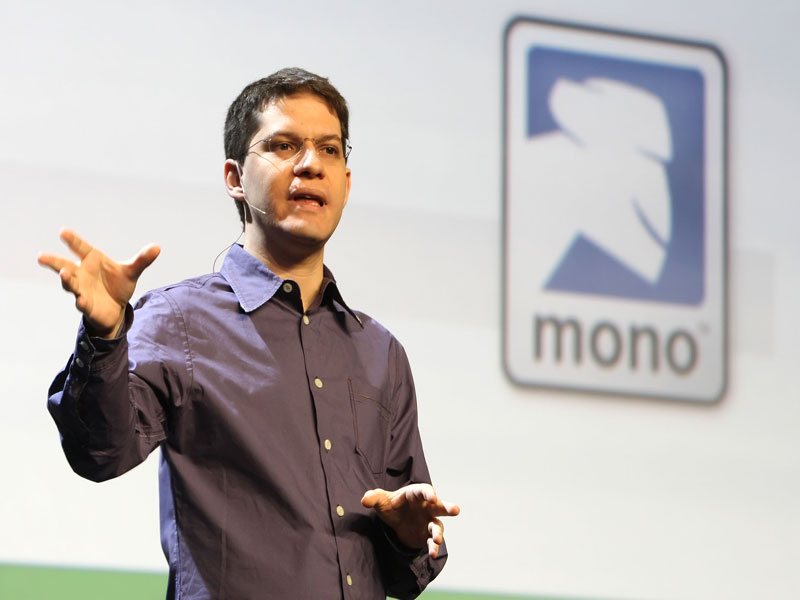
\includegraphics[height=1.80in]{figs/miguel_de_icaza.jpg}
%  \caption{{\footnotesize Linus Torvalds}}
\end{center}
\end{figure}

\pause

\begin{center}
{\it Miguel de Icaza}
\end{center}

\end{frame}

%%%%%%%%%%%%%%%%%%%%%%%%%%%%%%%%%%%%%%%%%%%%%%%%%%%%%%%%%%%%%%
\begin{frame}
\frametitle{FLOSS Leader}

Some ideas to find information about this leader.
\pause
\begin{itemize}
\item A short bio.
\item Initial contributions of Miguel to Linux and other open source projects.
\item The desktop conceived by Miguel and others.
\item Enterprises.
\item How is he making a living today?
\item \ldots
\end{itemize}

\end{frame}

%%%%%%%%%%%%%%%%%%%%%%%%%%%%%%%%%%%%%%%%%%%%%%%%%%%%%%%%%%%%%%
%%%%%%%%%%%%%%%%%%%%%%%%%%%%%%%%%%%%%%%%%%%%%%%%%%%%%%%%%%%%%%
%%%%%%%%%%%%%%%%%%%%%%%%%%%%%%%%%%%%%%%%%%%%%%%%%%%%%%%%%%%%%%
\begin{frame}
\frametitle{FLOSS Leader}

\begin{figure}[h]
\begin{center}
  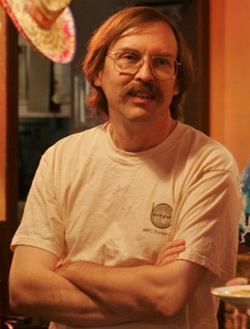
\includegraphics[height=1.80in]{figs/larry_wall.jpg}
%  \caption{{\footnotesize Linus Torvalds}}
\end{center}
\end{figure}

\pause

\begin{center}
{\it Larry Wall}
\end{center}

\end{frame}

%%%%%%%%%%%%%%%%%%%%%%%%%%%%%%%%%%%%%%%%%%%%%%%%%%%%%%%%%%%%%%
\begin{frame}
\frametitle{FLOSS Leader}

Some ideas to find information about this leader.
\pause
\begin{itemize}
\item A short bio.
\item The importance of Perl in the history of Internet.
\item Other projects he has created or contributed.
\item How is he making a living today?
\item \ldots
\end{itemize}

\end{frame}

%%%%%%%%%%%%%%%%%%%%%%%%%%%%%%%%%%%%%%%%%%%%%%%%%%%%%%%%%%%%%%
\begin{frame}
\frametitle{FLOSS Leader}

\begin{figure}[h]
\begin{center}
  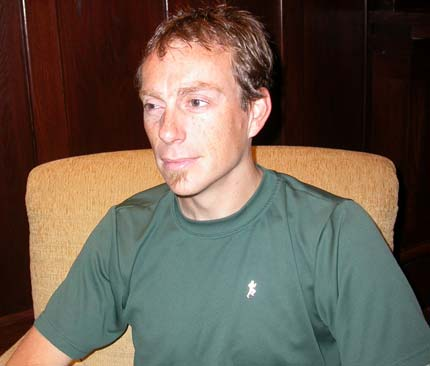
\includegraphics[height=1.80in]{figs/theo_de_raadt.jpg}
%  \caption{{\footnotesize Theo De Raadt}}
\end{center}
\end{figure}

\pause

\begin{center}
{\it Theo de Raadt}
\end{center}

\end{frame}

%%%%%%%%%%%%%%%%%%%%%%%%%%%%%%%%%%%%%%%%%%%%%%%%%%%%%%%%%%%%%%
\begin{frame}
\frametitle{FLOSS Leader}

Some ideas to find information about this leader.
\pause
\begin{itemize}
\item A short bio.
\item The importance of BSD Unix in the history of Internet.
\item Projects he has founded, leadered or contributed.
\item Libre software drivers advocacy.
\item Controversies with NetBSD and Linux developers.
\item How is he making a living today?
\item \ldots
\end{itemize}

\end{frame}

%%%%%%%%%%%%%%%%%%%%%%%%%%%%%%%%%%%%%%%%%%%%%%%%%%%%%%%%%%%%%%
%%%%%%%%%%%%%%%%%%%%%%%%%%%%%%%%%%%%%%%%%%%%%%%%%%%%%%%%%%%%%%
\begin{frame}
\frametitle{FLOSS Leader}

\begin{figure}[h]
\begin{center}
  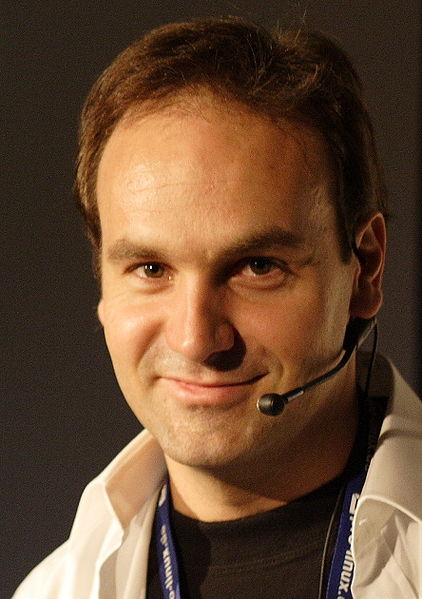
\includegraphics[height=1.80in]{figs/Mark_Shuttleworth.jpg}
%  \caption{{\footnotesize Mark Shuttleworth}}
\end{center}
\end{figure}

\pause

\begin{center}
{\it Mark Shuttleworth}
\end{center}

\end{frame}

%%%%%%%%%%%%%%%%%%%%%%%%%%%%%%%%%%%%%%%%%%%%%%%%%%%%%%%%%%%%%%
\begin{frame}
\frametitle{FLOSS Leader}

Some ideas to find information about this leader.
\pause
\begin{itemize}
\item A short bio.
\item What is Ubuntu? And what was the origin of the name?
\item Relationship with the Debian project.
\item The art of release.
\item How is he making a living today?
\item \ldots
\end{itemize}

\end{frame}

%% http://www.markshuttleworth.com/archives/146

%%%%%%%%%%%%%%%%%%%%%%%%%%%%%%%%%%%%%%%%%%%%%%%%%%%%%%%%%%%%%%
%%%%%%%%%%%%%%%%%%%%%%%%%%%%%%%%%%%%%%%%%%%%%%%%%%%%%%%%%%%%%%
\begin{frame}
\frametitle{FLOSS Leader}

\begin{figure}[h]
\begin{center}
  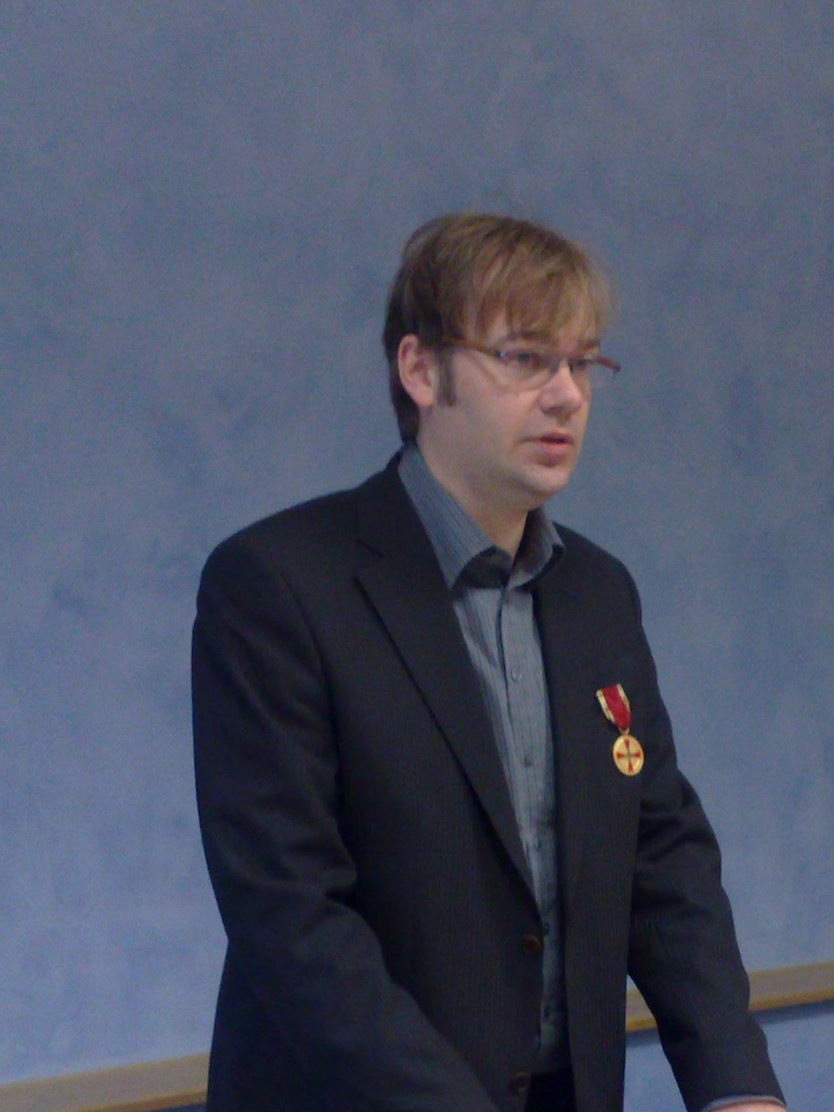
\includegraphics[height=1.80in]{figs/Matthias_Ettrich.jpg}
%  \caption{{\footnotesize Matthias Ettrich}}
\end{center}
\end{figure}

\pause

\begin{center}
{\it Matthias Ettrich}
\end{center}

\end{frame}

%%%%%%%%%%%%%%%%%%%%%%%%%%%%%%%%%%%%%%%%%%%%%%%%%%%%%%%%%%%%%%

\begin{frame}
\frametitle{FLOSS Leader}

Some ideas to find information about this leader.
\pause
\begin{itemize}
\item A short bio.
\item What is KDE? And what was the origin of the name?
\item Contributions to other libre software projects 
\item How is he making a living today?
\end{itemize}

\end{frame}


%%%%%%%%%%%%%%%%%%%%%%%%%%%%%%%%%%%%%%%%%%%%%%%%%%%%%%%%%%%%%%
%%%%%%%%%%%%%%%%%%%%%%%%%%%%%%%%%%%%%%%%%%%%%%%%%%%%%%%%%%%%%%
\begin{frame}
\frametitle{FLOSS Leader}

\begin{figure}[h]
\begin{center}
  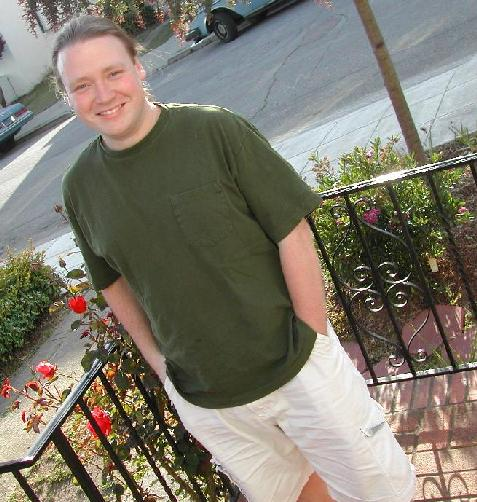
\includegraphics[height=1.80in]{figs/Brian_Behlendorf.jpg}
%  \caption{{\footnotesize Brian Behlendorf}
\end{center}
\end{figure}

\pause

\begin{center}
{\it Brian Behlendorf}
\end{center}

\end{frame}

%%%%%%%%%%%%%%%%%%%%%%%%%%%%%%%%%%%%%%%%%%%%%%%%%%%%%%%%%%%%%%
\begin{frame}
\frametitle{FLOSS Leader}

Some ideas to find information about this leader.
\pause
\begin{itemize}
\item A short bio.
\item The Apache server project and the ASF
\item Involment in other Open Source projects 
\item How is he making a living today?
\item \ldots
\end{itemize}

\end{frame}

%%%%%%%%%%%%%%%%%%%%%%%%%%%%%%%%%%%%%%%%%%%%%%%%%%%%%%%%%%%%%%

%%%%%%%%%%%%%%%%%%%%%%%%%%%%%%%%%%%%%%%%%%%%%%%%%%%%%%%%%%%%%%
%% Otras personas
%% Alan Cox
%% Bruce Perens
%% Ian Murdock
%% Miguel de Icaza
%% Larry Wall
%% Michael Widenius and David Axmark (MySQL)
%% Larry Augustin (SugarCRM, Geeknet...)
%% Hans Reiser (ReiserFS, historia con morbo CSI :) )
%%
%% Cuatro por bloque.
%% Repartido en grupos ...
%% La sesión cubrirá 2 horas hablando de 4 líderes.
%%
%%%%%%%%%%%%%%%%%%%%%%%%%%%%%%%%%%%%%%%%%%%%%%%%%%%%%%%%%%%%%%

\section{About Opensistemas}

%%%%%%%%%%%%%%%%%%%%%%%%%%%%%%%%%%%%%%%%%%%%%%%%%%%%%%%%%%%%%%

\begin{frame}
\frametitle{About Opensistemas}
\begin{center}
Opensistemas is an {\LARGE international} company \pause highly {\LARGE specialized} \pause in
offering global {\Huge IT solutions} \pause based on {\Huge Open Source} and {\Huge Linux} platforms.
\end{center}
\end{frame}

\begin{frame}
\frametitle{About Opensistemas}
\begin{itemize}
\item Our Vision:
\pause
To become the international leader in Open Source Technologies.
\pause
\item Our Mission:
\pause
Apply our knowledge of the opportunities offered by Open Source to deliver
effective solutions and innovation to our customers while promoting the
professional development of our employees and building value for 
shareholders.
\pause
\item Our Values:
\pause
\begin{itemize}
\item Deliver effective solutiosn to our customers.
\item Corporate social responsibility.
\item Commitment to Open Source.
\item Ethics and Respect for individuals.
\item Research and Innovation.
\item Teamwork.
\item Commitment to the development of a society connected by information
and knowledge.
\end{itemize}
\end{itemize}
\end{frame}

\begin{frame}
\frametitle{About Opensistemas}
\begin{center}
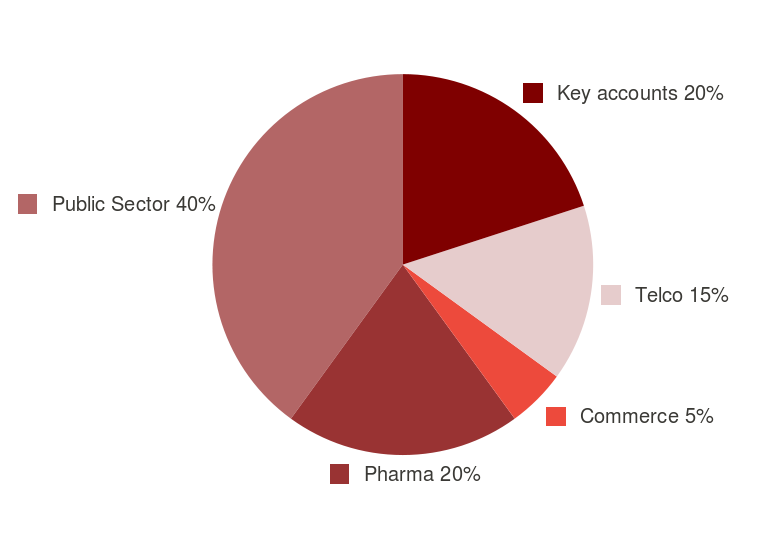
\includegraphics[width=9cm]{figs/opensistemas-markets}
\end{center}
\begin{center}
Our Markets
\end{center}
\end{frame}

\begin{frame}
\frametitle{About Opensistemas}
\begin{center}
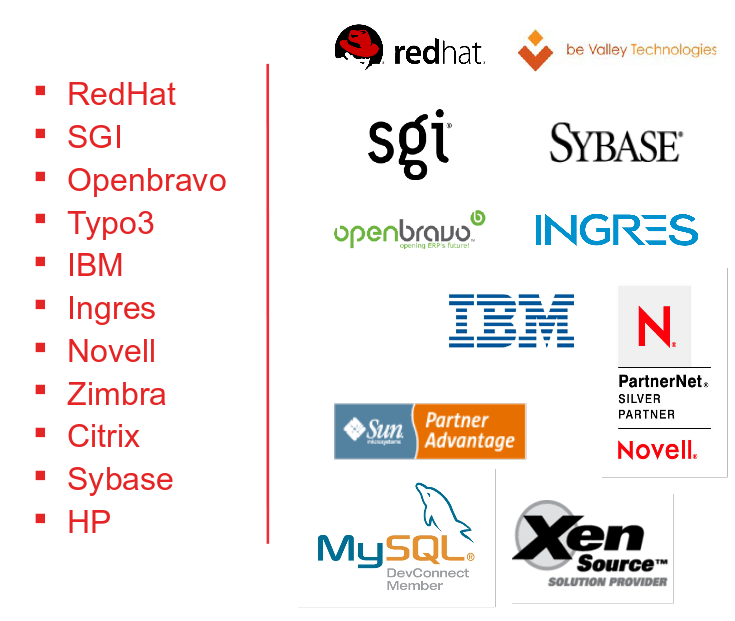
\includegraphics[width=7cm]{figs/opensistemas-partners}
\end{center}
\begin{center}
Our Partners
\end{center}
\end{frame}

\begin{frame}

\frametitle{About Opensistemas}
\begin{center}
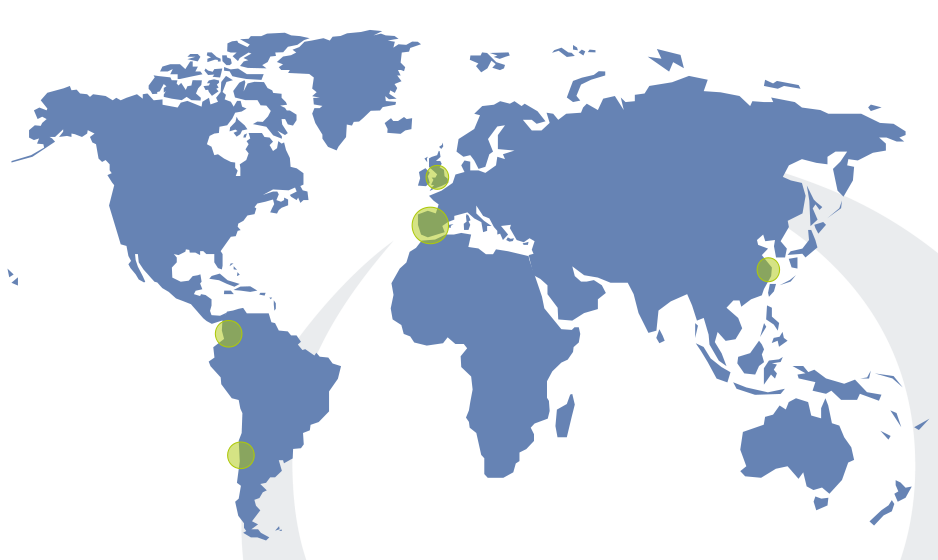
\includegraphics[width=9cm]{figs/opensistemas-worldmap}
\end{center}
\begin{center}
{\small Opensistemas is present in nine locations over five countries: Spain (Madrid, Valencia, Barcelona, Sevilla, Zaragoza), Chile (Santiago), Colombia (Bogotá), United Kingdom (London) and China (Shanghai).}
\end{center}
\end{frame}

\begin{frame}

\frametitle{About Opensistemas}
{\Huge Contact Information}
\begin{itemize}
\item www.opensistemas.com
\item info@opensistemas.com
\item +34 902 107 396
\end{itemize}
\end{frame}

\end{document}
